\chapter{提案手法}
\label{chap:implementation_and_experimentation}

\section{Omnet++とDTNsimを用いた評価環境}
\label{section:Omnet++とDTNsimを用いた評価環境}
Omnet++はネットワークシミュレータの構築を目的としたオープンソースのプラットフォームであり, 
既存の通信プロトコルや物理層のシミュレーションを実装しているほか, 
各ノードにC++でのアプリケーションを実装し拡張することが可能である. 
DTNsimはOmnet++のフレームワーク上で動作するDTNのシミュレーターであり, 
ION-DTN, HDTNなどの種々のDTN実装が動作するネットワークをシミュレートすることができ, 
各種CGRのバリエーションにも対応する. そのため本研究ではこのOmnet++とDTNsimを用いて
宇宙で運用されているDTNをシミュレーションを行う. 

\section{2030・2040年代のDTNを想定したシミュレーション}
\label{section:2030・2040年代のDTNを想定したシミュレーション}
本実験においては, 2030年代に地球・月間, 2040年代に地球・月・火星間にまたがるDTNを運用していることを想定し, 
そのうち任意の2天体間について既存手法と本研究の提案手法の実装とシミュレーションを行い, 
本研究の提案の有効性について検証する. そのため任意の2天体間のDTNネットワークとして, 
図\ref{fig:experimentation_topology}と同様のトポロジーを想定する. 

\ref{section:2030年代の地球・月間のDTNを想定したシミュレーションのシナリオとパラメータ}項では
2030年代の地球・月間のDTNにおけるシナリオ, 
\ref{section:2040年代の地球・月・火星間のDTNを想定したシミュレーションのシナリオとパラメータ}項では
2040年代の地球・月・火星間のDTNにおけるシナリオを説明する. 

\subsection{2030年代の地球・月間のDTNを想定したシミュレーションのシナリオとパラメータ}
\label{section:2030年代の地球・月間のDTNを想定したシミュレーションのシナリオとパラメータ}
2030年代の人類の月における活動区域は当面月の南極域になることが予想され, 
図\ref{fig:artemis_moon_station_orbit}に示すように, 
月南極域との通信可能時間の長いNRHO軌道の利用が検討されている. 
本実験ではこのNRHO軌道を利用した地球・月間のDTNネットワークを想定し, 
図\ref{fig:experimentation_topology}のトポロジーにおいて, 
それぞれ以下の構成を用いる. 

\begin{table}[htbp]
    \centering
    \caption{地球・月間シナリオのトポロジーと図\ref{fig:experimentation_topology}での表示の対応関係}
    \begin{tabular}{cc}  \hline
        図\ref{fig:experimentation_topology}での表示 & 本シナリオにおける対応 \\ \hline
        天体A & 地球 \\
        天体B & 月 \\
        ノード1 & 地球の地上DTNノード \\
        ノード2 & 地球の静止軌道上に存在するDTNノード \\
        ノード3 & 地球の静止軌道上に存在するDTNノード \\
        ノード4 & 月のNRHO軌道上に存在するDTNノード \\
        ノード5 & 月のNRHO軌道上に存在するDTNノード \\
        ノード6 & 月の地表DTNノード \\ \hline
    \end{tabular}
    \label{table:earth_moon_scenario_topology}
\end{table}

地球の静止軌道上に存在するDTNノードは地球に対してほぼ円軌道を描き, 
地表からおよそ36,000km(およそ0.12光秒)の高度を飛行する. 
また月のNRHO軌道上に存在するDTNノードは,  
月面から4,000km(およそ0.01光秒)$\sim$75,000km(およそ0.25光秒)程度を極端な楕円軌道を描いて飛行する. 
そのため地球の静止軌道上に存在するDTNノードと月のNRHO軌道上に存在するDTNノードの距離について
図\ref{fig:distance_earth_moon}のように考えられる. 
これらを考慮し, シミュレーションにおけるノード間の距離は表\ref{table:earth_moon_scenario_distance}のように設定した. 
% \begin{figure}[tbh]
%     \centering
%     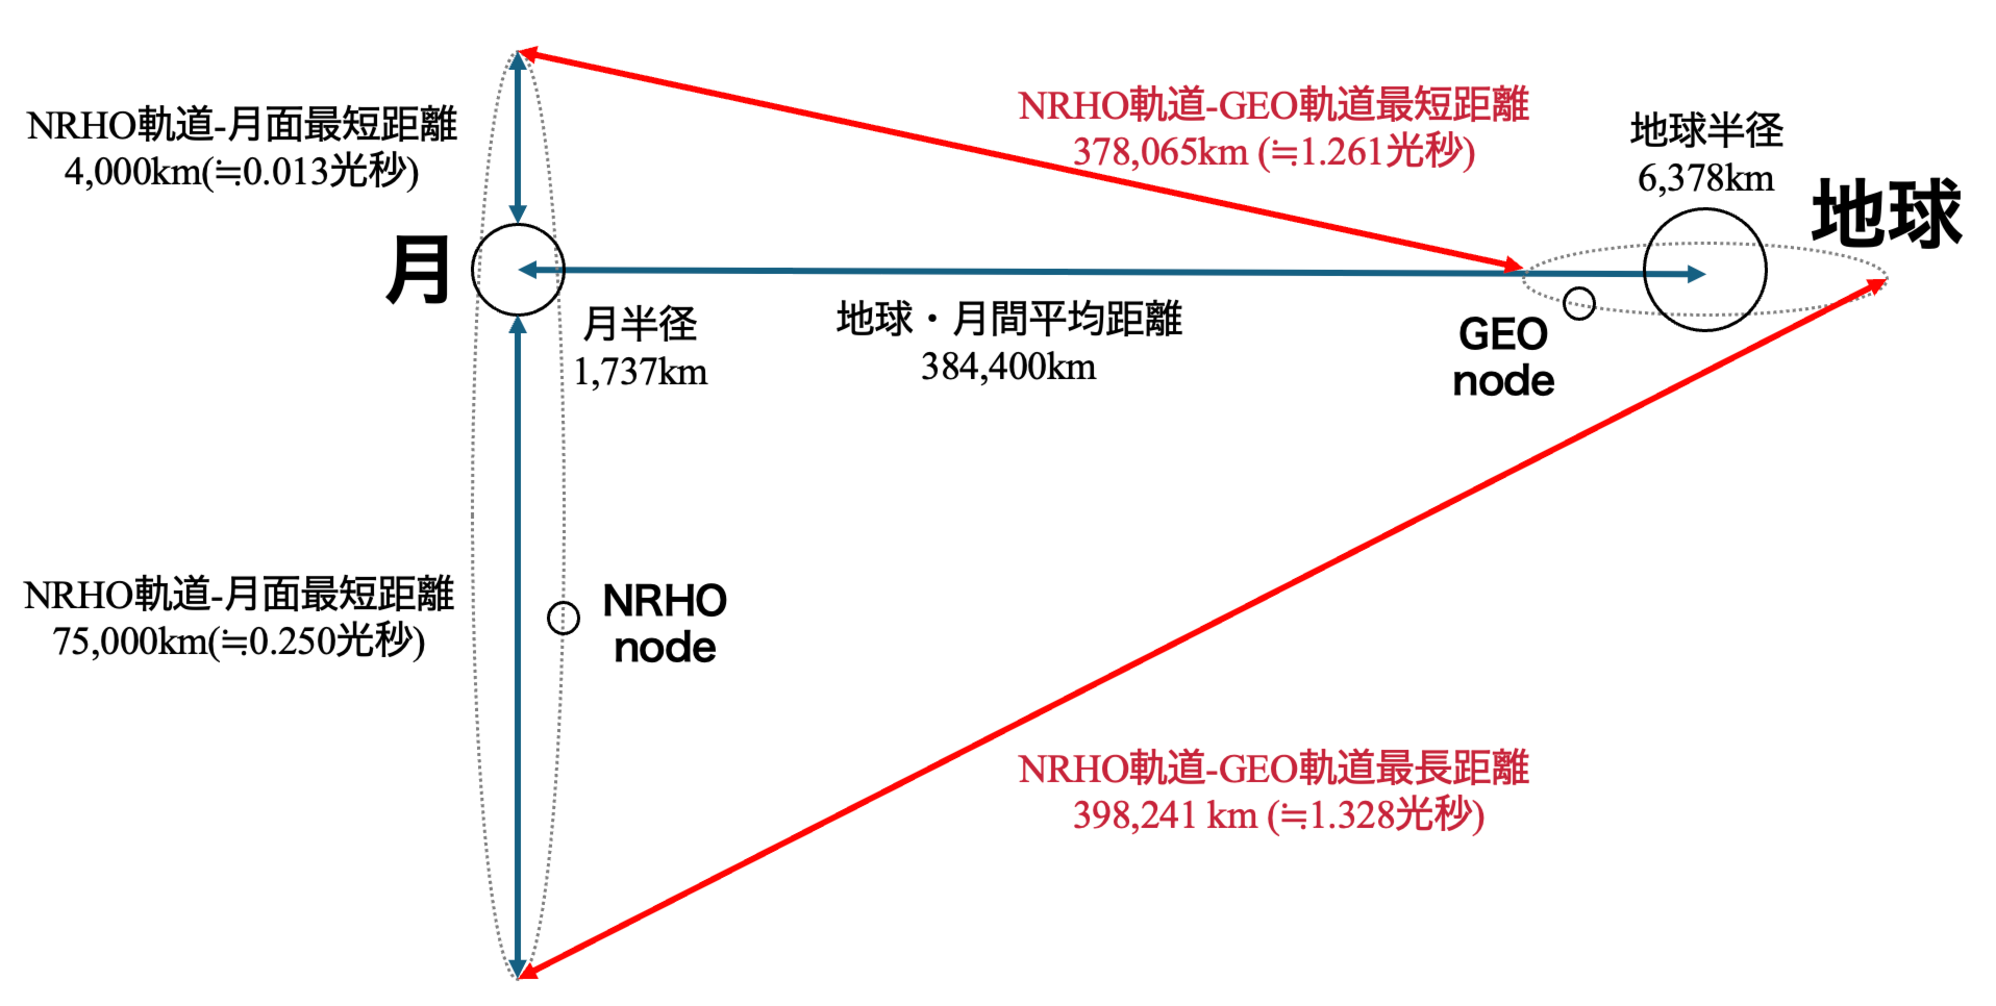
\includegraphics[width=0.7\textheight]{img/simulation_params_earth_moon.pdf}
%     \caption{地球・月間シナリオにおけるノード間の距離の概要}
%     \label{fig:distance_earth_moon}
% \end{figure}

\begin{table}[htbp]
    \centering
    \caption{地球・月間シナリオのシミュレーションに用いる各ノード間の距離}
    \begin{tabular}{cc}  \hline
        図\ref{fig:experimentation_topology}でのノードペア & Contact Planに表記する距離 \\ \hline
        ノード1 - ノード2またはノード3 間 & 0.12光秒 \\
        ノード2 - ノード3 間 & 0.37光秒 \\
        ノード2またはノード3 - ノード4またはノード5  間 & 1.29光秒 \pm15\% \\
        ノード4 - ノード5  間 & 0.14光秒 \pm 50\% \\
        ノード4またはノード5 - ノード6  間 & 0.13光秒 \pm 92\% \\ \hline
    \end{tabular}
    \label{table:earth_moon_scenario_distance}
\end{table}

\subsection{2040年代の地球・月・火星間のDTNを想定したシミュレーションのシナリオとパラメータ}
\label{section:2040年代の地球・月・火星間のDTNを想定したシミュレーションのシナリオとパラメータ}
2040年代には活動区域は火星にまで広がっていることが予想される. 
火星における運用計画等は現時点では未定ではあるものの, 
PhobosとDeimosを利用した軌道上の基地の設置なども構想されている.
そのため本実験では表\ref{table:earth_mars_scenario_topology}のように
地球・火星間のDTNネットワークを想定する. 

\begin{table}[htbp]
    \centering
    \caption{地球・火星間シナリオのトポロジーと図\ref{fig:experimentation_topology}での表示の対応関係}
    \begin{tabular}{cc}  \hline
        図\ref{fig:experimentation_topology}での表示 & 本シナリオにおける対応 \\ \hline
        天体A & 地球 \\
        天体B & 月 \\
        ノード1 & 地球の地上DTNノード \\
        ノード2 & 地球の静止軌道上に存在するDTNノード \\
        ノード3 & 地球の静止軌道上に存在するDTNノード \\
        ノード4 & Phobosの近傍に存在するDTNノード \\
        ノード5 & Deimosの近傍に存在するDTNノード \\
        ノード6 & 火星の地表DTNノード \\ \hline
    \end{tabular}
    \label{table:earth_mars_scenario_topology}
\end{table}

この時, 地球・火星・Phobos・Deimos間の距離は図\ref{fig:distance_earth_mars}のような値を用いることでおおよその値が推定ができる. 
また地球と火星間の距離の変動周期が非常に長いため, 200光秒・750光秒・1300光秒の3つの値を用いてそれぞれ別にシミュレーションを行った.
地球と火星間の距離が200光秒の時のシミュレーションにおけるノード間の距離を表\ref{table:earth_mars_scenario_distance_200}のように, 
750光秒の時のシミュレーションにおけるノード間の距離を表\ref{table:earth_mars_scenario_distance_750}のように, 
1300光秒の時のシミュレーションにおけるノード間の距離を表\ref{table:earth_mars_scenario_distance_1300}のように設定した.


% \begin{figure}[tbh]
%     \centering
%     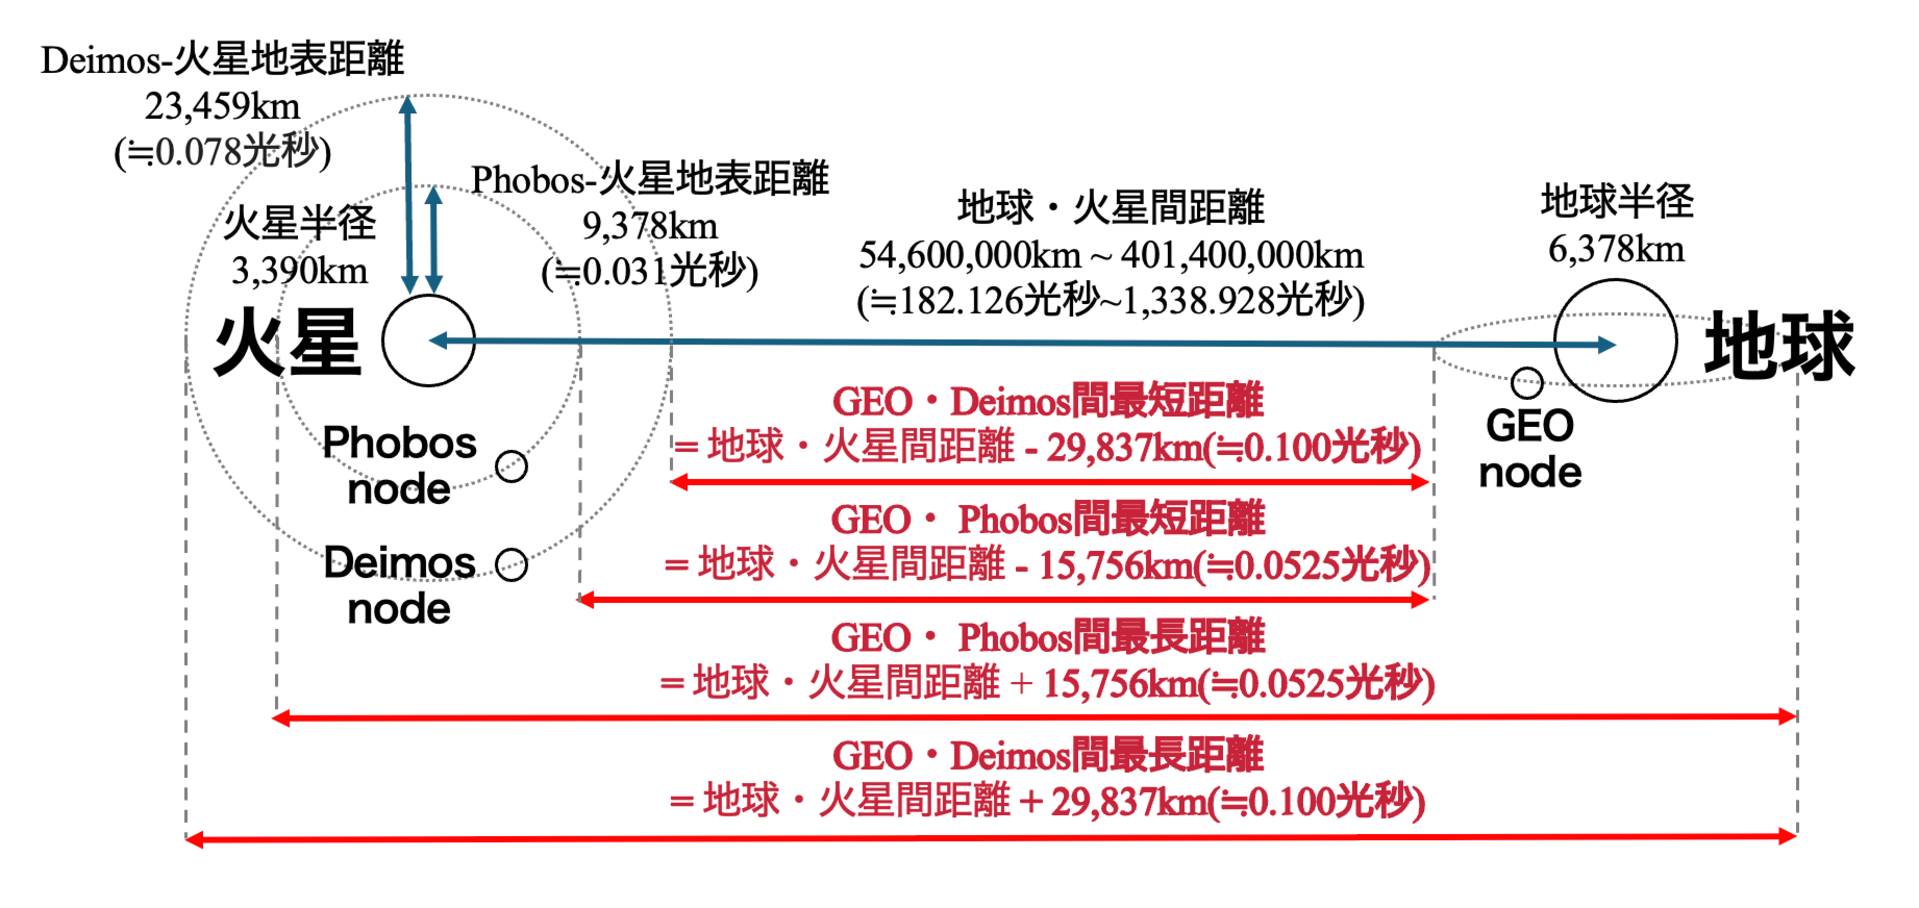
\includegraphics[width=0.7\textheight]{img/simulation_params_earth_mars.pdf}
%     \caption{地球・月・火星間シナリオにおけるノード間の距離の概要}
%     \label{fig:distance_earth_mars}
%     \begin{minipage}{\textwidth}
%         \raggedright
%         \fontsize{10.5pt}\selectfont
%     \end{minipage}
% \end{figure}

\begin{table}[htbp]
    \centering
        \caption{地球・月・火星間シナリオのシミュレーションに用いる各ノード間の距離 \\(地球・火星間の距離が200光秒のシナリオ)}
    \begin{tabular}{cc}  \hline
        図\ref{fig:experimentation_topology}でのノードペア & Contact Planに表記する距離 \\ \hline
        ノード1 - ノード2またはノード3 間 & 0.12光秒 \\
        ノード2 - ノード3 間 & 0.37光秒 \\
        ノード2またはノード3 - ノード4  間 & 200光秒 \pm0.050\% \\
        ノード2またはノード3 - ノード5  間 & 200光秒 \pm0.026\% \\
        ノード4 - ノード5  間 & 0.078光秒 \pm40\% \\
        ノード4 - ノード6  間 & 0.031光秒 \\ 
        ノード5 - ノード6  間 & 0.078光秒 \\ \hline
    \end{tabular}
    \label{table:earth_mars_scenario_distance_200}
\end{table}
\begin{table}[htbp]
    \centering
        \caption{地球・月・火星間シナリオのシミュレーションに用いる各ノード間の距離 \\(地球・火星間の距離が750光秒のシナリオ)}
    \begin{tabular}{cc}  \hline
        図\ref{fig:experimentation_topology}でのノードペア & Contact Planに表記する距離 \\ \hline
        ノード1 - ノード2またはノード3 間 & 0.12光秒 \\
        ノード2 - ノード3 間 & 0.37光秒 \\
        ノード2またはノード3 - ノード4  間 & 750光秒 \pm0.013\% \\
        ノード2またはノード3 - ノード5  間 & 750光秒 \pm0.007\% \\
        ノード4 - ノード5  間 & 0.078光秒 \pm40\% \\
        ノード4 - ノード6  間 & 0.031光秒 \\ 
        ノード5 - ノード6  間 & 0.078光秒 \\ \hline
    \end{tabular}
    \label{table:earth_mars_scenario_distance_750}
\end{table}
\begin{table}[htbp]
    \centering
        \caption{地球・月・火星間シナリオのシミュレーションに用いる各ノード間の距離 \\(地球・火星間の距離が1300光秒のシナリオ)}
    \begin{tabular}{cc}  \hline
        図\ref{fig:experimentation_topology}でのノードペア & Contact Planに表記する距離 \\ \hline
        ノード1 - ノード2またはノード3 間 & 0.12光秒 \\
        ノード2 - ノード3 間 & 0.37光秒 \\
        ノード2またはノード3 - ノード4  間 & 1300光秒 \pm0.007\% \\
        ノード2またはノード3 - ノード5  間 & 1300光秒 \pm0.004\% \\
        ノード4 - ノード5  間 & 0.078光秒 \pm40\% \\
        ノード4 - ノード6  間 & 0.031光秒 \\ 
        ノード5 - ノード6  間 & 0.078光秒 \\ \hline
    \end{tabular}
    \label{table:earth_mars_scenario_distance_1300}
\end{table}
\subsection{シミュレーションで用いるBundleトラフィック}
\label{section:シミュレーションで用いるBundleトラフィック}
本実験では図\ref{fig:experimentation_topology}のトポロジーにおいて, 
ノード1からノード6に向かう, すなわち天体Aの地上DTNネットワークから天体Bの地上DTNネットワークに
向けてのトラフィックを想定する. DTNsimではトラフィックとして生成するBundleについて様々な
パラメータを設定することが可能である. 本論文におけるシミュレーションではそれぞれ
表\ref{table:traffic_earth_moon}と表\ref{table:traffic_earth_mars}の値を用いた. 
また実際の宇宙インターネットにおけるトラフィックの発生状況は当然時刻変動するものであるが, 
本論文におけるシミュレーションでは単位時間あたりのトラフィック量は概ね一定であると仮定した.

\begin{table}[htbp]
    \centering
    \caption{地球・月間シナリオのトポロジーと図\ref{fig:experimentation_topology}での表示の対応関係}
    \begin{tabular}{ccc}  \hline
        図\ref{fig:experimentation_topology}での表示 & パラメータ名 & 値 \\ \hline
        シミュレーション全体におけるBundleの総生成数 & bundlesNumber & 1800 \\
        生成したBundleの送信元ノードのendpoint ID & sourceEid & 1 \\
        生成したBundleの宛先ノードのendpoint ID & destinationEid & 6 \\
        Bundle生成イベントごとのBundleのサイズ(bytes)& size & 1500\\
        Bundle生成イベントの間隔(秒)& interval & 1 \\ \hline
    \end{tabular}
    \label{table:traffic_earth_moon}
\end{table}

\begin{table}[htbp]
    \centering
    \caption{地球・火星間シナリオのトポロジーと図\ref{fig:experimentation_topology}での表示の対応関係}
    \begin{tabular}{ccc}  \hline
        図\ref{fig:experimentation_topology}での表示 & パラメータ名 & 値 \\ \hline
        シミュレーション全体におけるBundleの総生成数 & bundlesNumber & 8000 \\
        生成したBundleの送信元ノードのendpoint ID & sourceEid & 1 \\
        生成したBundleの宛先ノードのendpoint ID & destinationEid & 6 \\
        Bundle生成イベントごとのBundleのサイズ(bytes)& size & 1500\\
        Bundle生成イベントの間隔(秒)& interval & 10 \\ \hline
    \end{tabular}
    \label{table:traffic_earth_mars}
\end{table}
